%!TEX root = ../thesis.tex
%*******************************************************************************
%*********************************** First Chapter *****************************
%*******************************************************************************

\chapter{Background}  %Title of the First Chapter

\ifpdf
    \graphicspath{{Chapter1/Figs/Raster/}{Chapter1/Figs/PDF/}{Chapter1/Figs/}}
\else
    \graphicspath{{Chapter1/Figs/Vector/}{Chapter1/Figs/}}
\fi


%********************************** %First Section  **************************************
%\section{What is loren ipsum? Title with math \texorpdfstring{$\sigma$}{[sigma]}} %Section - 1.1 
\section{Motivation}



Increased human populations during the industrialisation of the 19th century were accompanied by increasing amounts of unmanaged waste that resulted in public health problems. The first attempts at remedying the issues where applied mostly to running waters, and had a bacteriological focus \cite{AQUATIC_INSECTS_BIOMONITORING}. As time passed, managing freshwater systems became more important and evolved into a more complex procedure that took into account entire aquatic communities (like macro-invertebrates and fish) rather than specific species. Animals inhabiting the system studied were used as indicators of sources of pollution that could no have been identified by chemical analysis. Thus, the link between environmental management and biological monitoring came as response to the needs of human populations.



Nearing the end of the 20th century, "ecological health" became a priority in some human societies; people begun pressuring public authorities to restore freshwater systems to a healthier state. This is also reflected in the political sphere with the rise of Green parties in more economically developed nations across the world. Subsequently, huge budgets have been allocated in the management of freshwater, and other, systems; an example being the restoration of the Emscher river system which has an estimated cost of US\$5.5billion \cite{emscher}. 

 The driving motive today for the assessment of environmental consequences (from plans, policies or projects) around the world is coming from regional legislation, operations of Non-Governmental Organisations and requirements set by the financial backers of projects in the area. Legal procedures, policies and instruments are set up to ensure that decision makers take into consideration the environmental impacts of their projects; examples include the Environmental Impact Assessment Directive of the European Union \cite{eia_eu} and the Environmental Protection Agency in the United States \cite{us_epa_our_2013}, both of which became operational around the 1970s.
 
 

Environmental studies conducted all around the world test sites such as fish farms (for example in New Zealand, Scotland, Norway and others) \cite{stoeck_environmental_2018}, rivers that cross various landscapes, land (used for dairy-farming, horticulture, or where different kinds of forests grow)\cite{hermans_bacteria_2016} and many others. A good way to infer the health of an environment is by investigating the species inhabiting it, and in particular their relative abundance\footnote{Species abundance is the number of individuals comprising a species in a particular area. Relative abundance is how individuals in a community are distributed among species.}; some species are very intolerant of pollution (Alderfly Larva) whereas others are tolerant (Leeches, Blood Worms). Thus, the distribution of individuals in the various species (or other higher taxonomic groups) can tell us a lot about the levels of pollution. 

The method of using species as indicators to survey the health of an environment is called biomonitoring. The discipline's aim is to find the ideal bioindicators whose presence or behaviour reflects best a stressor's effect on biota. As an example, in rivers, the quality of water can be assessed by examining macro-invertebrates, fishes \cite{bioindicatorsinrivers}, and bacterial communities \cite{stoeck_environmental_2018} found at different sites. In land, soil bacterial community composition can be used to infer soil condition and health \cite{hermans_bacteria_2016}.

%Explaining current methods of biomonitoring
%taxonomic
The traditional methods of biomonitoring involve a limited, long-scaled site sampling of individual organisms which are then processed and sorted into sample taxonomic units. This process can take months to years, and usually produces data of low information \cite{baird_biomonitoring_2012}. Analysis of ecosystems requires taxonomic expertise across many order and several phyla; species-level identification is hindered by problems arising from co-ordinating the inputs of several experts, and differences in taxonomic refinement. As a result, the identified taxa are often very few in numbers, and are usually the ones deemed as critical (indicator organisms), by experts, for the specific study\cite{cranston_biomonitoring_1990}. 

The resolution of identification (or `taxonomic penetration') stops, more often that not, to taxonomically higher categories (genus, family etc) than species. The reasons for the reduction of penetration are usually not made explicit; most often a more pragmatic approach is taken which seeks to determine individuals to the species level only if the ease of doing it and the time taken permits it \cite{cranston_biomonitoring_1990}. As a result, most of the species which are more difficult to identify are lumped together to larger categories, loosing information in the process. This is especially the case with specious groups of freshwater organisms that occupy the lower levels of the food web, even though they constitute most of the biodiversity in the System and thus have the greatest potential for response to stressors \cite{woodward_biomonitoring_21st}. For example, lumping together species of the Chironomidae genus, because of the difficulty in separating them, reduces the sensitivity of the biomonitoring scheme used \cite{ruse_classification_2010}.

%The health of the environment in a particular area is closely related to finding out their relative abundance might be necessary to evaluate the quality of their habitat. The traditional method of identifying species is morpho-taxonomic, which requires expert knowledge, is time consuming and thus expensive. 


\section{Genomics: A new hope?}
The morpho-taxonomic\footnote{Taxonomic assignment based only on the morphology of the organism. This involves only its form and structure (appearance), but not its functions.} identification of species has been the limiting step in biomonitoring efforts because of the short-supply of taxonomists and prohibitive costs in separating and identifying species. The invention in 1977 of Sanger-based DNA sequencing\footnote{Sequencing is the process by which the order of the Nucleotides (or four bases) in a sample of DNA are found.} which revolutionised all branches of the biological sciences, could not be used for environmental bulk samples because they contained potentially thousands of species, and separating them for sequencing was prohibitively difficult. 

However, DNA sequence-based analysis has enabled ecologists to answer questions they would not have been able to without such data. In particular with the advent of DNA barcoding in 2004 \cite{hebert_paul_d._n._biological_2003}, which is a technique of identifying species based on short DNA sequences, international efforts have been made to build a taxonomic reference library (Barcode of Life Initiative), and identify unknown speciments to the species-level by comparing their sequence to known ones already catalogued in a reference database \cite{savolainen_vincent_towards_2005}. 
% Despite that, reliance to the methods has been going on for decades despite recent advances in molecular microbiology which aimed at describing assemblages of soil bacteria. 

The emergence of Next-generation sequencing (NGS) platforms brought significant improvements in DNA sequencing technologies \cite{shendure_next-generation_2008}. The new platforms can deliver billions of sequence reads per single run, which is orders of magnitude better than traditional Sanger sequencing. As a result there has been a significant drop of sequencing costs per megabases that has been going over the last 2 decades. In particular, the cost of sequencing 1 megabase has gone from \$$10^4$ in 2001, to \$$10^2 - 10^3$ in 2007 and finally to less than \$$10^{-1}$ in 2019 \cite{sequencing_costs}. This, coupled with advancements in DNA- and RNA-based techniques in taxonomic identification \cite{baird_biomonitoring_2012} have made possible the application of metagenetics, the study of genetic material sourced directly from the environment, in ecological studies. 

Normal barcoding standards were designed with the purpose of identifying isolated specimens from intact DNA using Sanger sequencing, so are inapplicable to empirical ecological studies where the samples contain DNA from a mixture of related species \cite{taberlet_towards_2012}. To solve this problem DNA metabarcoding was developed and made possible by NGS techologies. It is a method for high-throughput multi species identification using degraded DNA found in the environment (eDNA) \cite{taberlet_towards_2012}. The method relies on barcode genes which mutate at a rate that makes them stable within a species but different when compared to other ones, and which are used for the purpose of species identification. Examples are the 16S rRNA and the Cytochrome Oxidase 1 \cite{hebert_paul_d._n._biological_2003} genes. 

After the DNA is extracted from an environmental sample, its barcode region needs to be amplified (multiplied millions of times) before it can be sequenced. This involves selecting the right primers \footnote{Short molecules which provide the starting point for DNA amplification (in other words specify the region to be multiplied)} for the targeted taxonomic groups and using PCR for the amplification. The amplified DNA is then sequenced on a high-throughput sequencing platform and the sequences are processed and classified into Operational Taxonomic Units (OTUs). 
%Nowadays, however, the term "OTU" is generally used in a different context and refers to clusters of (uncultivated or unknown) organisms, grouped by DNA sequence similarity of a specific taxonomic marker gene.[2] In other words, OTUs are pragmatic proxies for microbial "species" at different taxonomic levels, in the absence of traditional systems of biological classification as are available for macroscopic organisms. For several years, OTUs have been the most commonly used units of microbial diversity, especially when analysing small subunit 16S or 18S rRNA marker gene sequence datasets. \url{https://en.wikipedia.org/wiki/Operational_taxonomic_unit}
%\url{https://www.ncbi.nlm.nih.gov/pmc/articles/PMC1609233/}

OTUs are an intentionally vague term used to cluster sequences produced from  metabarcoding. Reads with a predetermined percentage of similarity (usually 97\%) between them are classified into the same OTU. Thus they are acting as a proxy to traditional `species'. The most abundant sequence of each OTU is assigned a taxonomy using reference databases. Most of the times, even when cross referencing the OTUs with a taxonomic library, a species-level identification is not available; errors in sequencing reads and the arbitrary cut-off similarity percentile are among some of the factors that prevent identification. However, this might not necessarily be a downside of the metabarcoding approach. OTUs can still act as informative indicators if they respond to environmental gradients and have characteristic signatures. 
These developments allowed scientists to overcome the bottleneck of morpho-taxonomic identification of species. 


An advantage of NGS platforms is that they can sequence DNA from multiple environmental samples, each made of potentially hundreds of species. The sequences clustered into an OTU, per sample, are counted and registered in an sample-OTU table. This can mean, for example, that in the first sample collected from the environment, 30 sequences belonging to OTU1 were read, 0 belonging to OTU2, 20435 in OTU3 and so on until all OTUs are considered. OTUs can be completely taxonomically identified (up to the species level), partly (up to a higher level) or not at all. 
%Metagenomics, the study of genetic material directly sourced from the environment, has the ability to revolutionise biomonitoring and bring a new era of massive ecological data generation.


%%Differences between sangers and NGS
%Explain DNA barcoding and reference libraries

%what was done (taxonomic identification) and what can be done
%Older biomonitoring techniques relied too much on expert opinion and on a limited number of easily identifiable taxa. The methodologies used were not scientific. MEasuring the relative abundance of these taxa is not enough to assess the quality of an environment, especially if it is done in isolation. The whole community has to be taken into account and the way the species interact to get a full picture. \textbf{tocite}{woodward}
% Segway to next generation sequencing 
%Dna sequencing technology has undergone impressive improvements over the last year, with the advent of next generation sequencing. High-throughput sequencing is orders of magnitude cheaper and faster than traditional sanger sequencing. This leap of in sequencing capacity can revolutionise a variety of scientific disciplines \textbf{cite shendure 2008}. One such application of NGS is the health evaluation of habitats. \textbf{cite taberlet 2012}

%\section{Metabarcoding}
%Bacteria can be used as bioindicators to determine health of environment. This can be done because bacterial communities respond to changes in soil more than differences in the climate or geography.  bacterial taxonomic groups respond differently to various soil atributes (pH, carbon-to-nitrogen rations, Olsen P\footnote{Measure of plant available phosphorous} etc). Thus, the relative abundance of specific taxa reflect the impact of specific anthropogenic activities on the environment, even when comparing soil samples across large geographical areas.\cite{hermans_bacteria_2016}
%
%benthic bacterial communities react in a
%similar way to the same environmental stressors as benthic macrofauna
%communities.(Stoeck 2018)
%How we can identify bioindicators 


%6229 have to reach 6729

\section{Data}
Our data were sampled from the Northern Peruvian rivers in collaboration with WWF Peru. They comprise of a sample-OTU table constructed from water samples collected along the rivers' length, and metadata provided by WWF Peru. The metadata include information on the location, water colour, area of the river, trip number, date of sampling, and details of the sample for some of them.
\subsection{Geography}
%Explain topography of river
The Northern Peruvian rivers of interest are made up of the Maranon River on the west, which is joined by its tributary, the Huallaga River. Together they join with the Ucayali River to form the Amazon River, which runs across South America to the Atlantic Ocean. In addition to these rivers, the tributaries of Napo and Tapiche were sampled. 

The Peruvian rivers' confluence has the largest annual water discharge rate into the Amazon, making it the mainstream  source. The Maranon river flows from the Andes Jungle and mountains, through Pongo de Manseriche, a gorge (narrow steep valley of hills or mountains with a river flowing through it) northwest of Peru. The Pongo is series of torrents, interspersed with rocks, and at points reaches a width of no more than 25m. It acts like a natural barrier between the Upper Part of the Maranon river and the rest of the area, making the fauna upstream potentially different from downstream. For the purposes of the project, the Maranon River has been split into three areas: Upper, Mid and Lower, with the Upper being behind the Pongo. 
%Maranon upper is behind a natural barrier that makes it distinct from the other rivers etc
%he Amazon River begins in the Andes Mountains at the west of the basin with its main tributary the Marañón River in Peru.
%Pongo de Manseriche is a gorge in northwest Peru. The Marañón River runs through this gorge (and water gap) before it reaches the Amazon Basin.

From the river samples collected, some came from white and others from black waters. White water rivers appear so because of suspended  sediment. They have a higher concentration of minerals (especially sodium, potassium, magnesium, calcium) than Black rivers and have a neutral pH, compared to the acidic of Black waters. The dark colour on the other hand comes from tannins leaching from decaying vegetation. These differences have important implications for the rivers' fauna, since some species cannot live in  environments with low concentrations of particular minerals. Thus it is expected that different animal communities will be found in these different environments. 

A plot of the samples collected along the rivers can be seen in Figure \ref{fig:graphmap}. The different colours represent the rivers, and the shapes the water colour. There is a clear imbalance in the numbers of black and white water samples and also in their spatial distribution. From the 164 samples collected, 143 are white and 21 black. All of the black water samples are found in the Eastern part of the river, and along Ucayali, Tapiche, Napo and Maranon lower. 

\begin{figure}
	\centering
	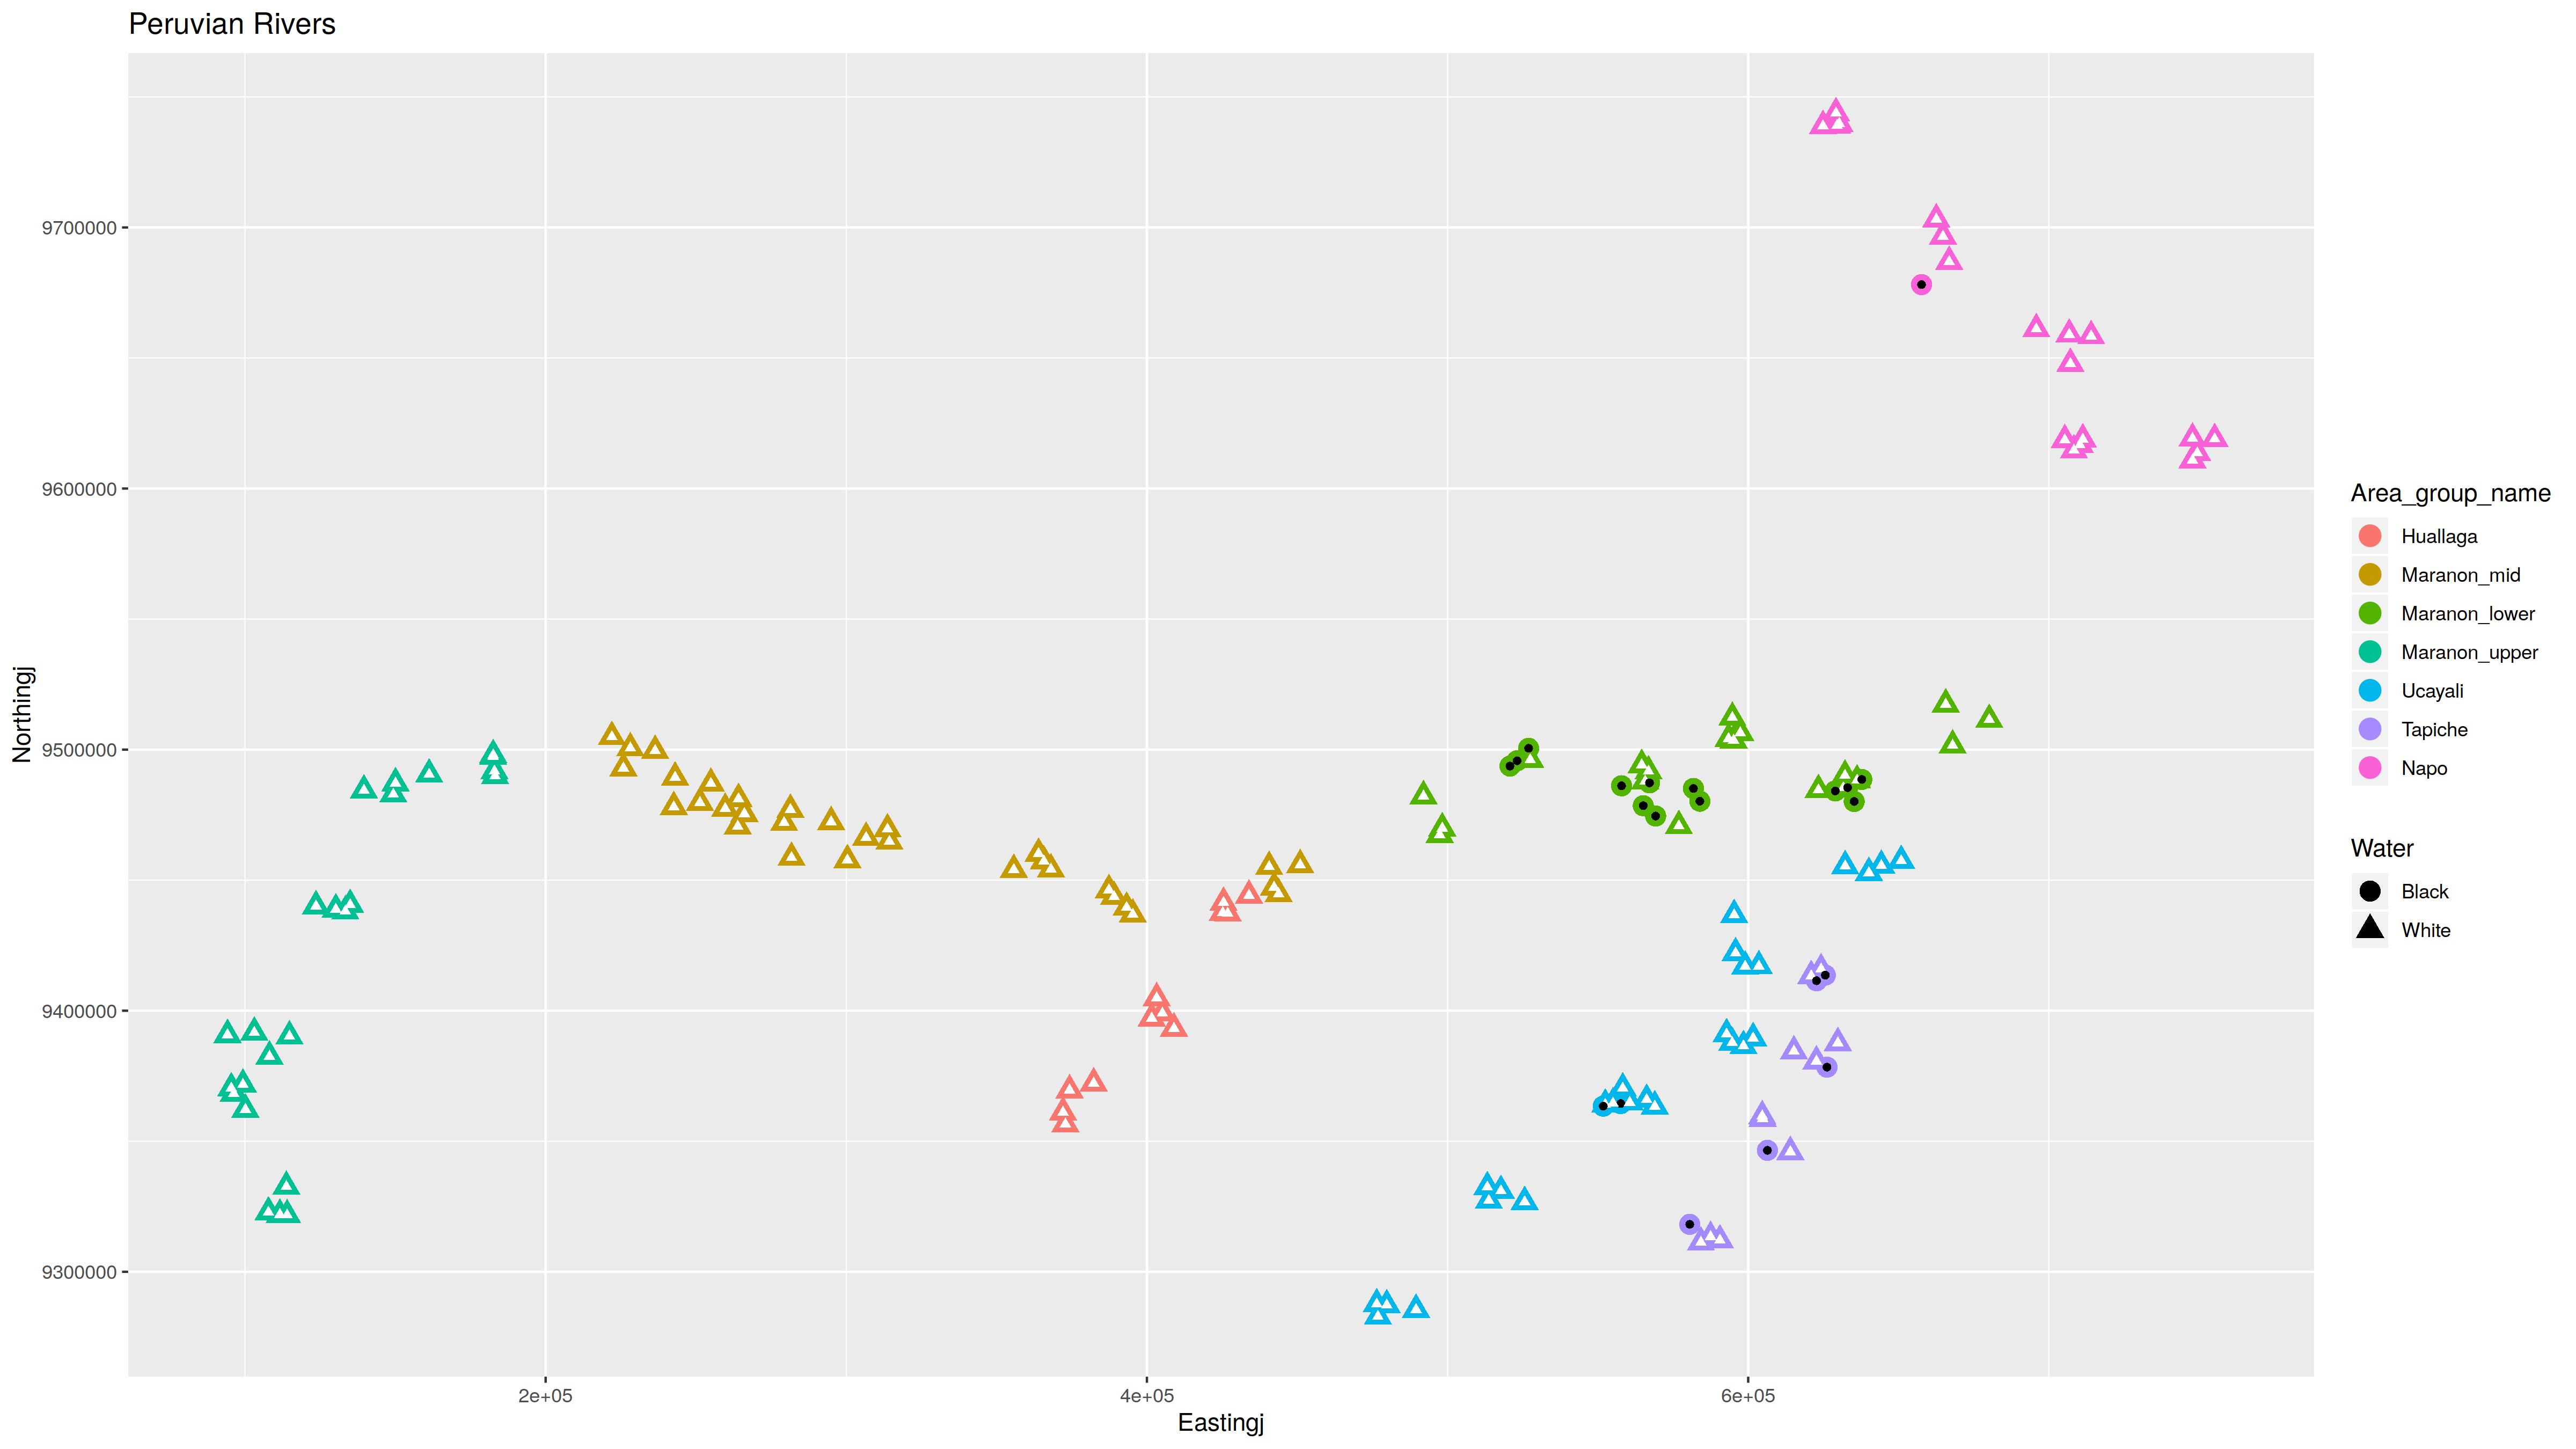
\includegraphics[width=0.7\textwidth]{mapofrivers}
	\caption{A plot of the Easting and Northing coordinates of the samples collected. Colours represent the rivers, and shapes the water colour (triangle for White and circle for Black). The points are also coloured white and black in the middle to aid in viewing. White noise with a standard deviation of $5 \cdot 10^3$ was added to the coordinates so as to separate points close together.}
	\label{fig:graphmap}
\end{figure}
\subsection{Sampling and Preprocessing}
%how data are sampled
The water samples were collected from the sides of a boat using kits provided by NatureMetrics. A volume of water, between 0.5-2L is filtered through a membrane which is then send to the laboratory for DNA extraction. From each site in the river (boat stop), 4 samples were collected (with some sites having a bit more). Information about the sites and samples was also recorded in the metadata (like ID, location, water colour, trip number and date of collection). 

At the laboratory, DNA trapped inside the membranes is extracted and then PCR amplified. The DNA fragments produced are then sequenced using high-throughput sequencing technology that can handle multiple samples at once. The raw reads from the sequencing are processed (filtered and assembled) and then clustered into OTUs with a similarity cut-off point of 99\%. The representative sequences, or the most abundant individual sequences per OTU, were used for taxonomic assignment. After removing the non identified OTUs we were left with 675 of them.

Five taxonomic Classes were kept for our analysis: Actinopterygii (fish), Amphibia, Aves (birds), Mammalia, and Reptilia. The most instances of OTUs found belonged to the Actinopterygii class, and within that, Siluriformes and Characiformes are the most abundant Orders. Class and Order distributions of OTUs can be seen in Figure \ref{fig:distr}. The sample-OTU table produced was very sparse (meaning that a significant number of entries were 0), as is the case for most studies using metabarcoding techniques. 
%PCR
%Next Generation sequencing
%Biases that come with sampling
%Removal of unidentified species
\begin{figure}[h]
	\centering
	\begin{subfigure}{0.45\textwidth}
		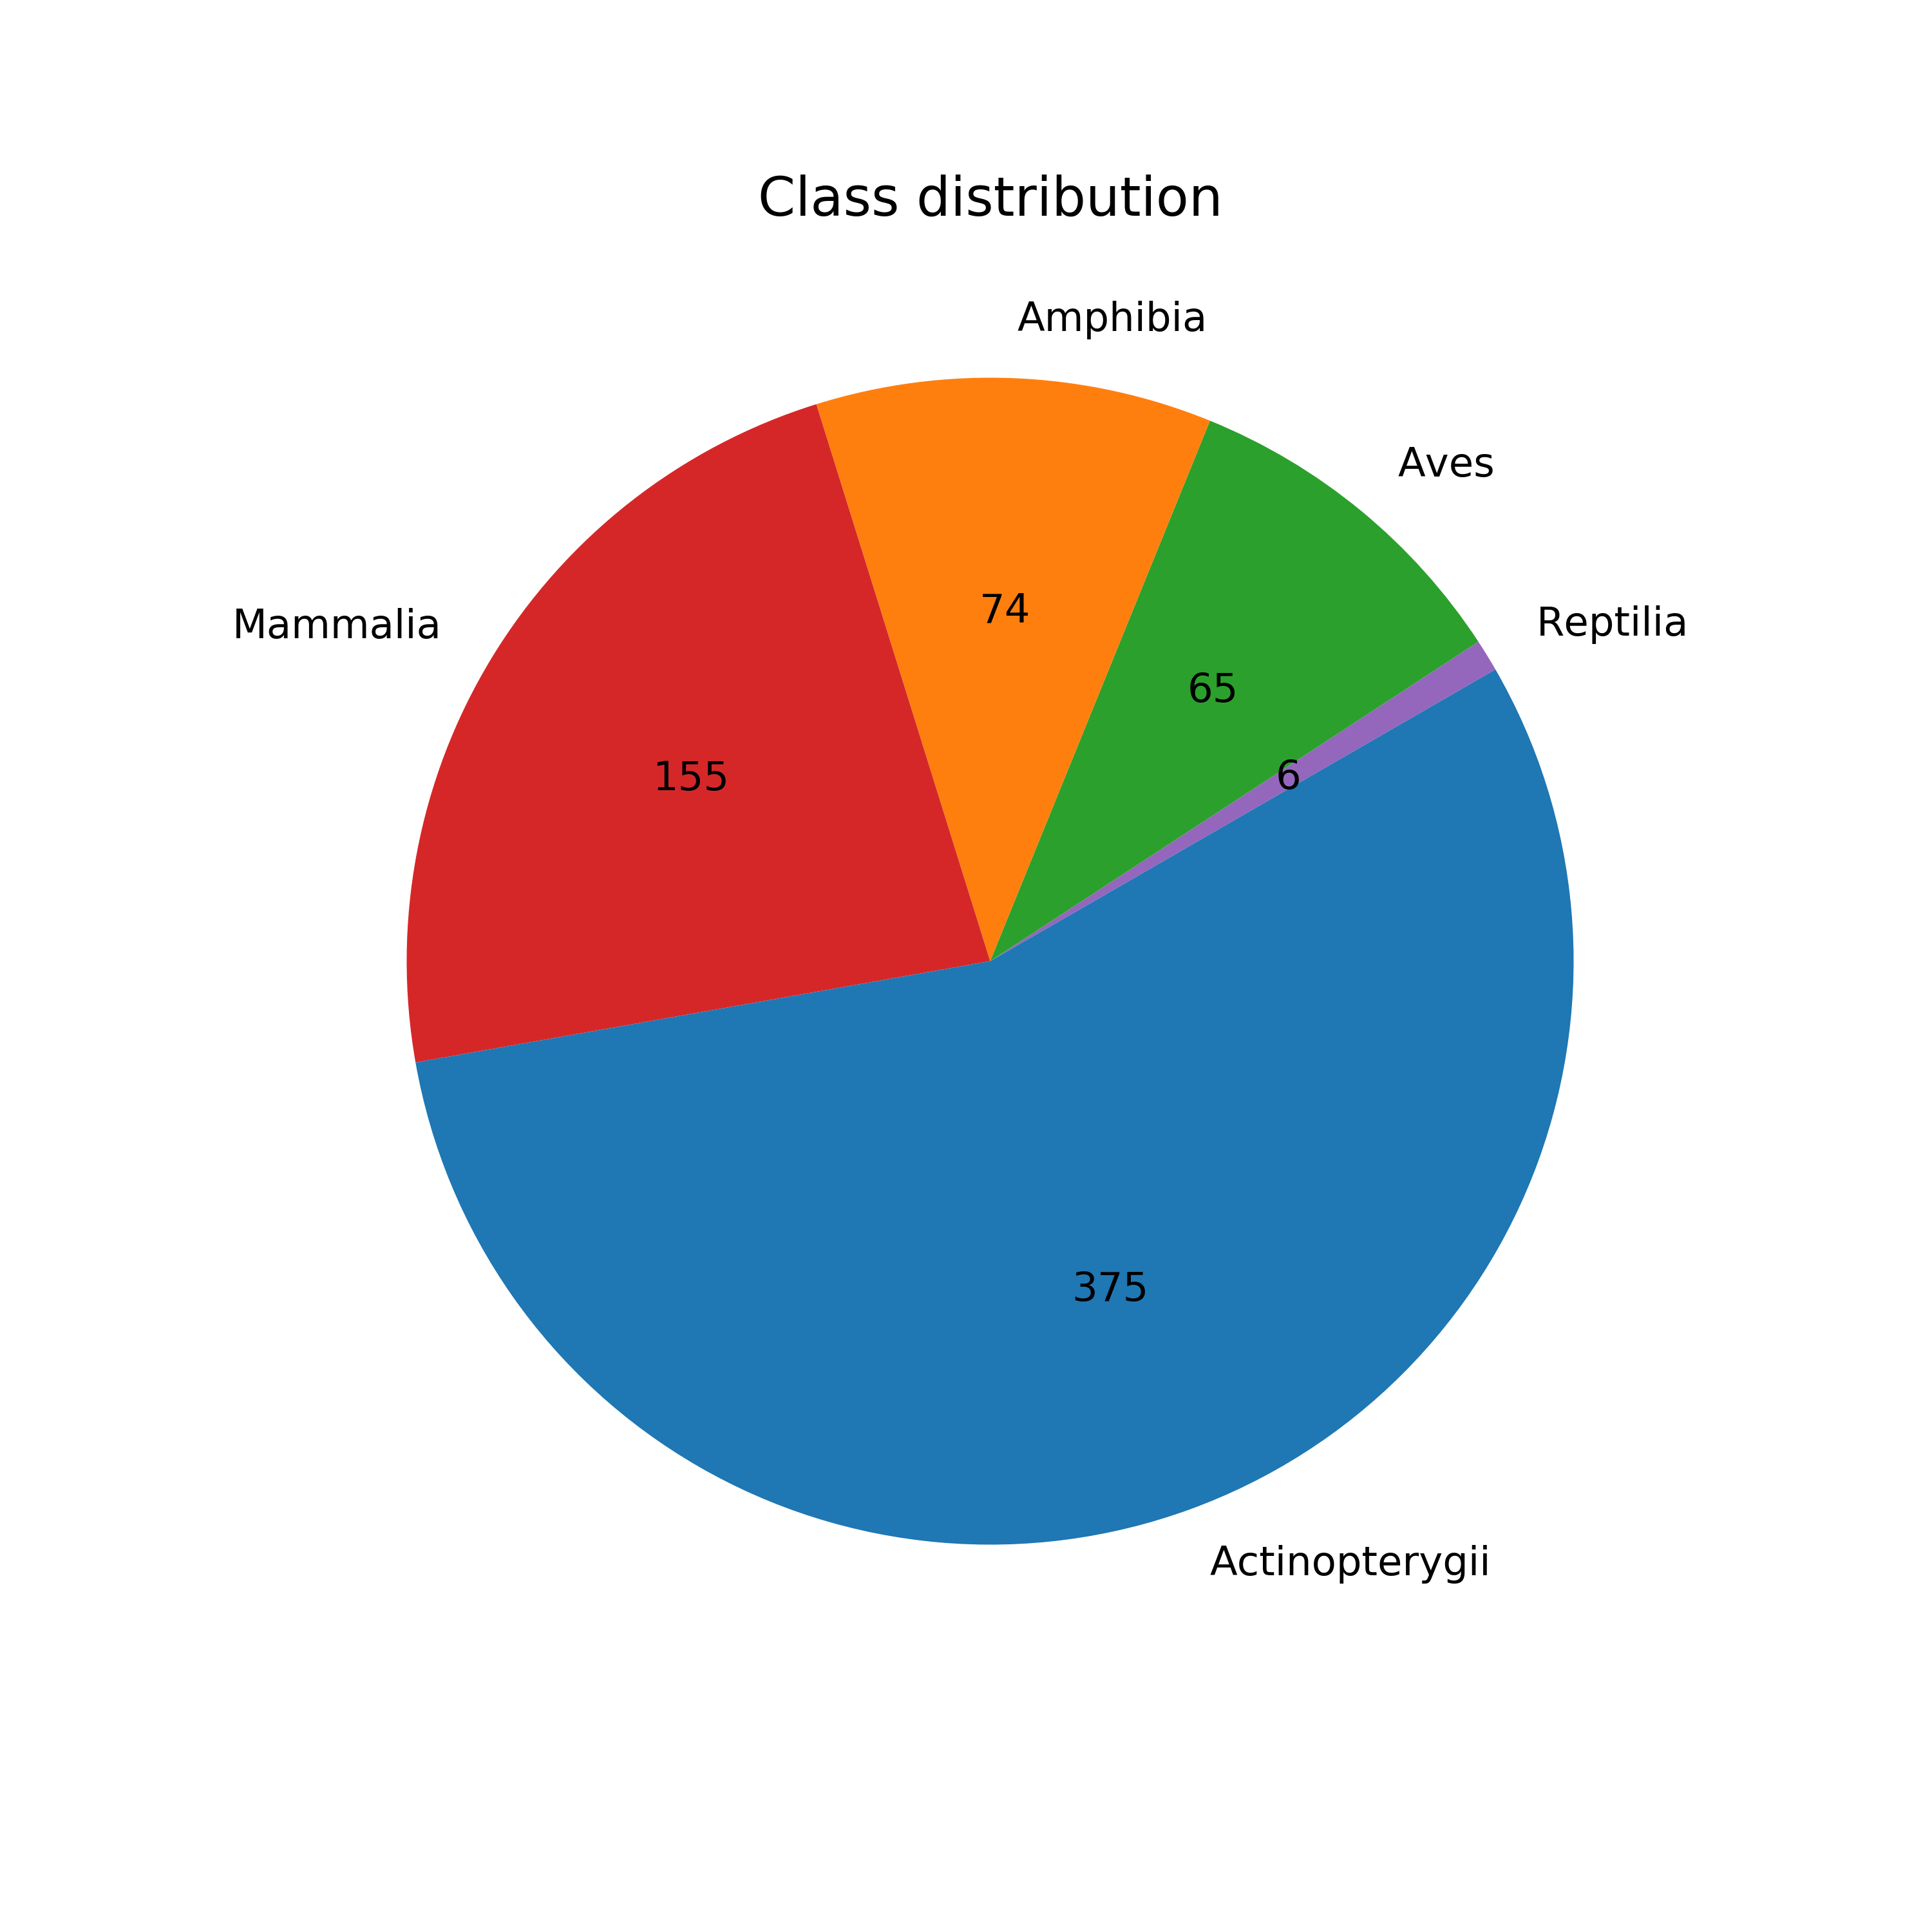
\includegraphics[width=\textwidth]{classdistrpie}
		\caption{Distribution of OTUs into Classes. Most abundant one is Actinopterygii.}
		\label{fig:classpie}
	\end{subfigure}
	\begin{subfigure}{0.45\textwidth}
		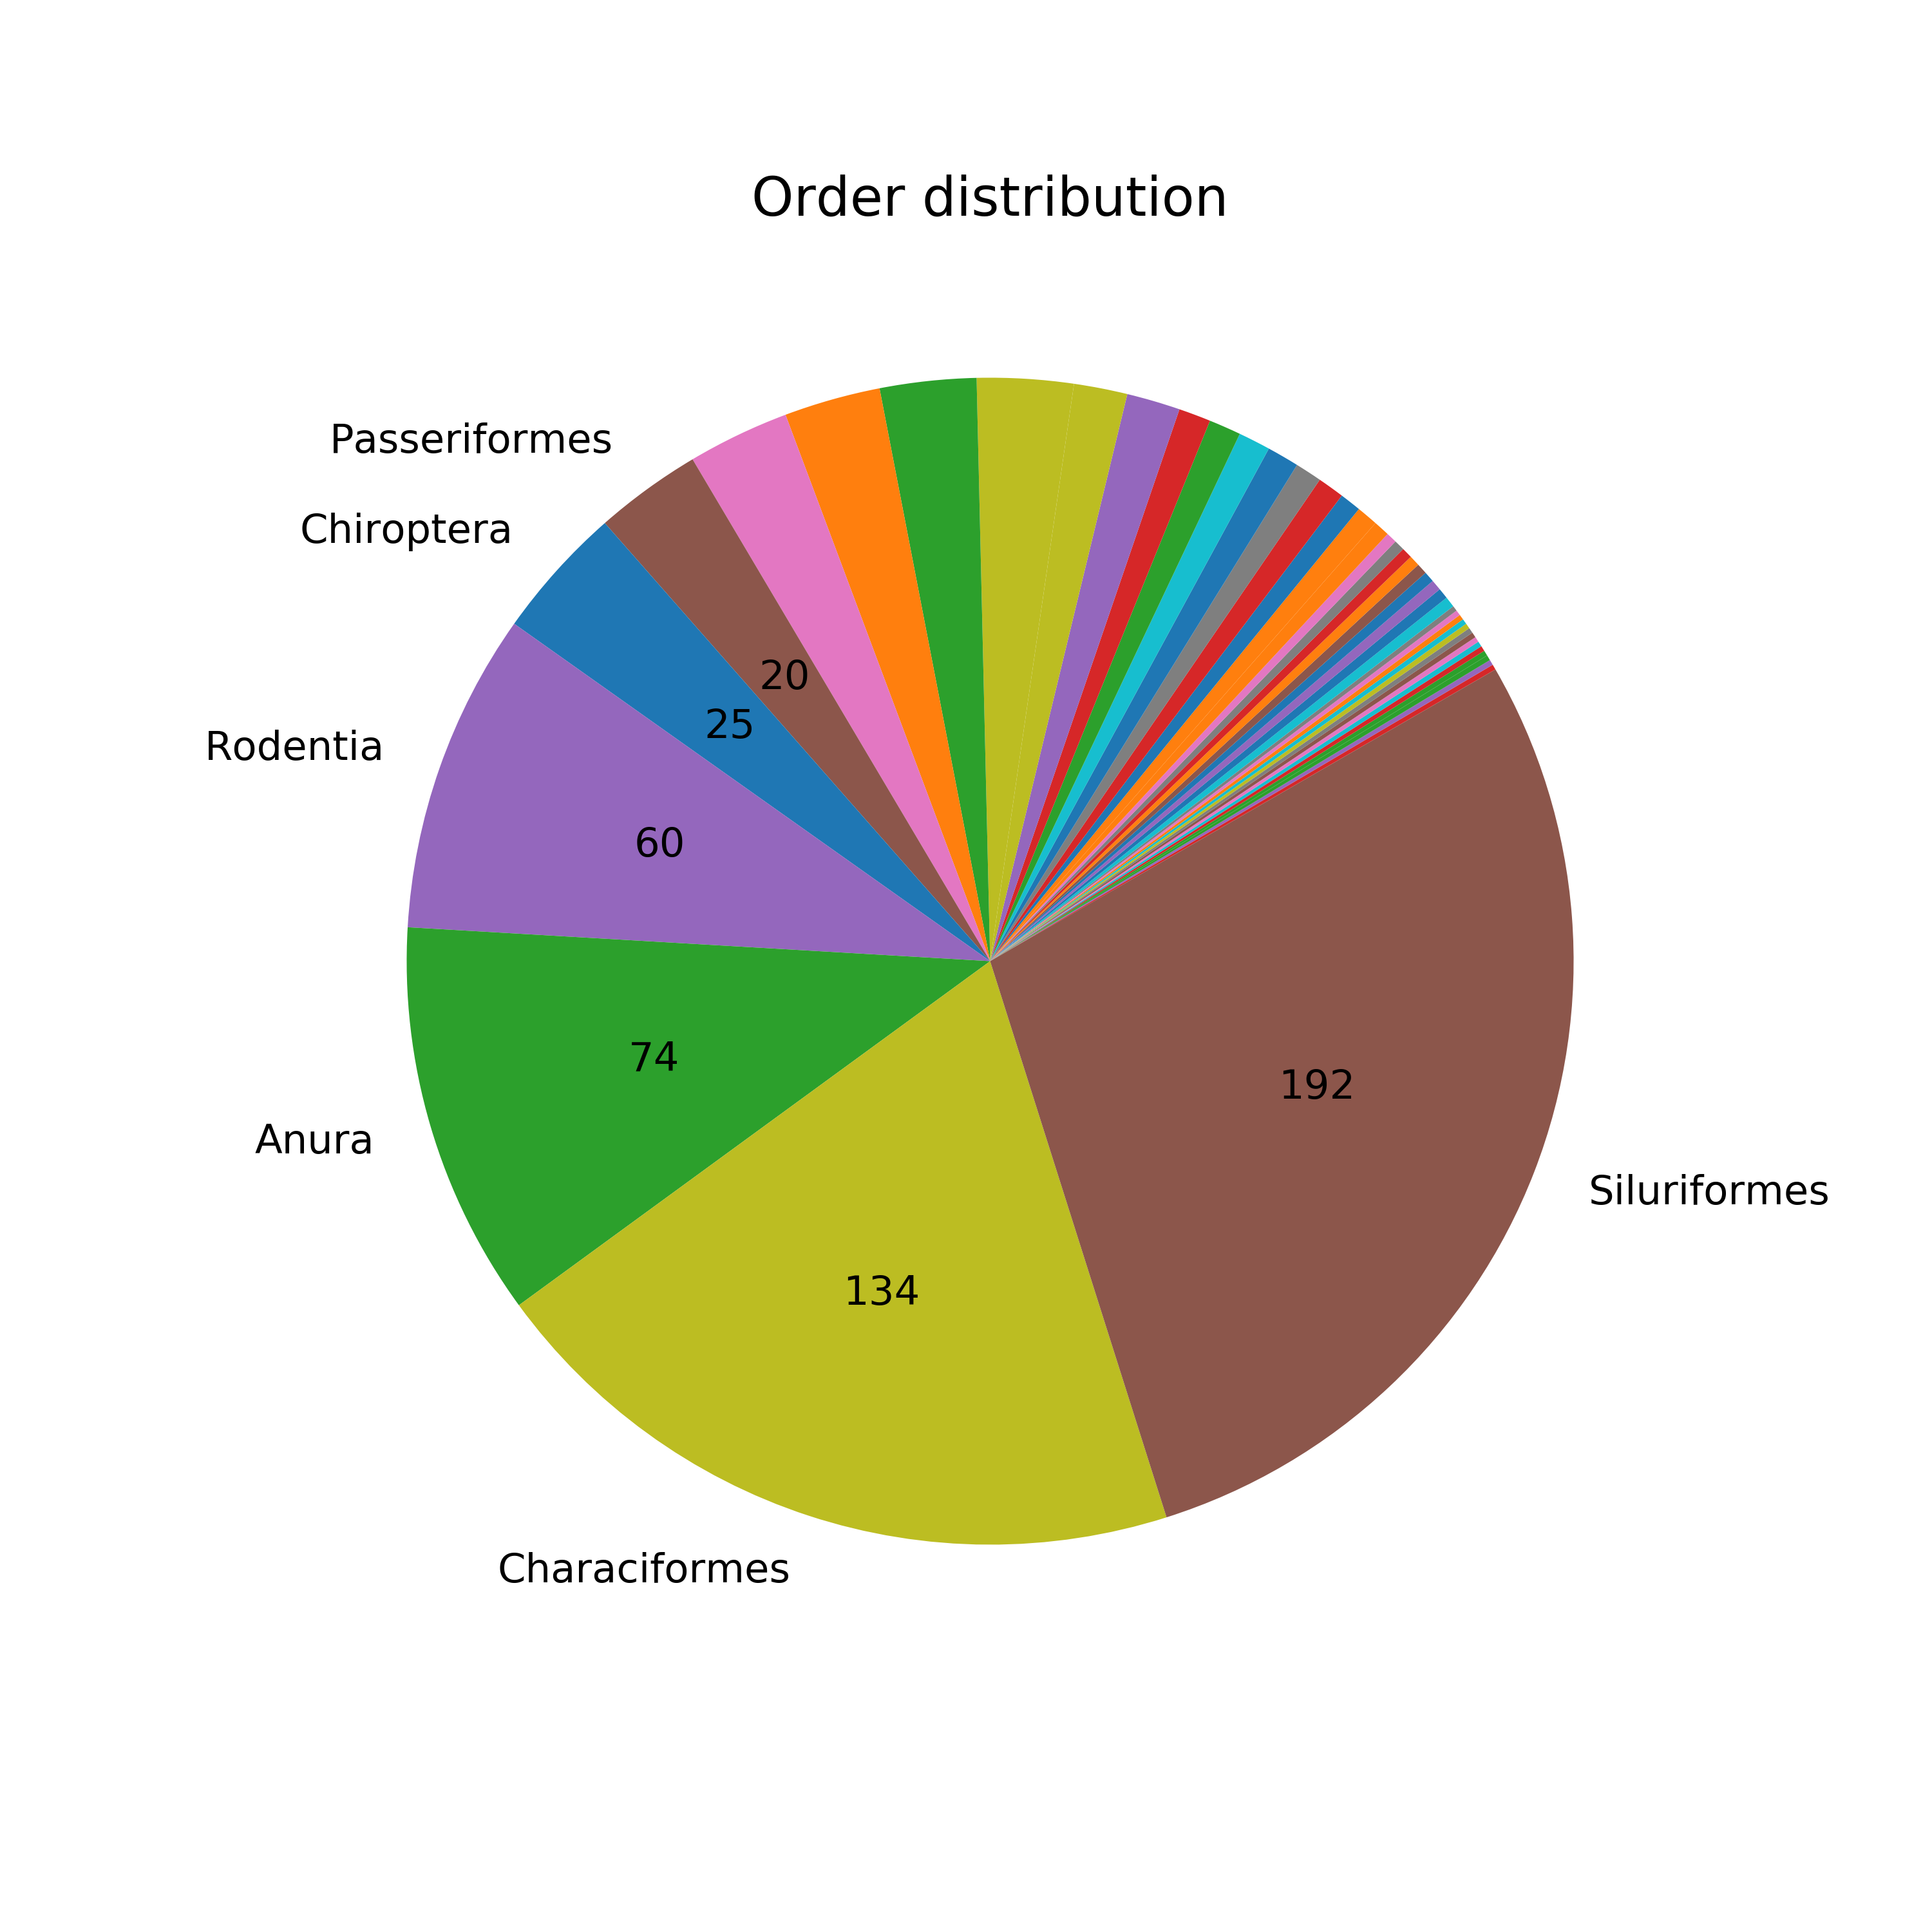
\includegraphics[width=\textwidth]{orderdistrpie}
		\caption{Distribution of OTUs into Orders. Most abundant ones are Siluriformes and Characiformes}
		\label{fig:orderpie}
	\end{subfigure}
\label{fig:distr}
\end{figure}

The sampling methods employed to produce our data come with some inherent biases. First of all, species give out different amounts, sizes and kinds of material behind that can be used to identify them. Furthermore, environmental DNA extracted from the samples can be PCR amplified at different rates for species. This can happen because of primer mismatch with the organisms barcode DNA region. This results in OTU reads that do not correlate well with the actual abundance of organisms in the environment and also to uninformative comparisons between OTUs' reads \cite{abundance_nodate}. 

Finally, the OTU table sparsity causes the reads to be concentrated on some samples only, with others having a much lower total read count (sum over the reads of all OTUs in a sample). There are 7 samples (all from white water parts of the river) with under 10000 total reads, of which 3 have less than 50. On the other hand, the sample with the largest total read counts has 219113 reads. 



\section{Literature Review}
%What has been done by others with data like ours
The advent of metagenetics has opened up the gateway for data driven research in multiple fields. From cataloguing micorbial genes in the human gut \cite{dos_santos_human_2010}, to ecological assessment of freshwater \cite{apotheloz-perret-gentil_taxonomy-free_2017} and river systems \cite{chariton_ecological_2010} using eDNA metabarcoding. Ecological monitoring has traditionally been done using the morpho-taxonomic identification of species in the environment studied. This involves identifying an organism up to a certain level and then using their presence in the site to come to conclusions about the health of the system.


Biotic indices are used to encapsulate information about the abundance of species identified in a site, and also indicate the degree to which a site is healthy. They are highly specialised in what type of pollution they can quantify and which species they consider as important \cite{washington_diversity_1984}. To calculate the value of a biotic index, the species found in a site are assigned a weight (or tolerance value) provided by the index and defined from empirical and experimental data \cite{borja_marine_2000}. Weights signify how susceptible an organism is to the pollution studied \cite{carter_chapter_2017}. Then an analytic formula uses the species weights to calculate the index's value which indicates the environmental quality of the system (usually in categories ranging from `very poor' to `very good').

As mentioned previously, the morpho-taxonomic identification of species is time consuming, expensive and limited in scope. Instead, a metabarcoding approach can generate an OTU table with assigned taxonomy from reference databases in significantly less time. The OTU reads can then be used to calculate biotic indices and evaluate the system's environmental health  \cite{lejzerowicz_high-throughput_2015}. Due to a lack of phylogenetic resolution and limited reference libraries, most metabarcoding data are not used in the calculation of indices. However, taxonomy-free approaches can be used to calculate proxies of biotic indices that have similar evaluation performance \cite{apotheloz-perret-gentil_taxonomy-free_2017}. 

One such approach to calculating biotic indices is through the use of supervised machine learning (SML). The first time that it was employed for biomonitoring surveys was in 2015 by Smith et al \cite{smith_natural_2015} (using microbial eDNA) and in 2017 by Cordier et al \cite{cordier_predicting_2017} (using eukaryotes eDNA). Cordier et al trained two SML models (Random Forests and Self Organising Map) to infer several Biotic Indices used often for marine studies. The features where OTUs reads obtained from foroamfinera eDNA sampled from the benthic zone (sediment on the bottom of the river) and processed in a similar way to the one outlined in the previous section. A notable difference is that unassigned OTUs (without taxonomy) were kept and used as features. Furthermore, the authors constructed new feature data sets using standard ecological techniques such as rarefying and alpha diversity metrics. Target values (biotic indices) were calculated using morpho-taxonomic data and associated weights. 

The SML models performed better in predicting the Biotic index of a site than a reference model that used the taxon assignments of OTUs and a correlation approach for assigning them weights. Also notable is that the SML models had a very high degree of agreement with the morpho-taxonomic evaluation of habitat quality. Furthermore, discarding low abundance OTUs (low total read counts across samples) did not affect the models' performance. The researchers followed up their paper with a more comprehensive one in 2018 \cite{cordier_supervised_2018}, which tested their SML methods on OTUs derived from 5 different ribosomal bacterial and eukaryotic markers\footnote{These markers are specifically designed to amplify regions of the genome that would be used in the identification of species. Multiple exist because of the different regions in the DNA needing to be amplified for the identification of specific groups of organisms (like eukaryotes and bacteria).}. They found that there was no significant difference in the models' performance when using different markers, and that for all of them, SML outperformed all taxonomy-based eDNA biomonitoring methods. 



Usually, analysis of metabarcoding (OTU reads per sample) or metagenetic (genes per sample) studies does not involve machine learning approaches. Researchers analyse alpha (within) and beta (between) diversity metrics of samples (see Figure \ref{fig:otu}), explore the patterns in beta diversity using ordination techniques, and perform various classical hypothesis tests. 

\begin{figure}
	\centering
	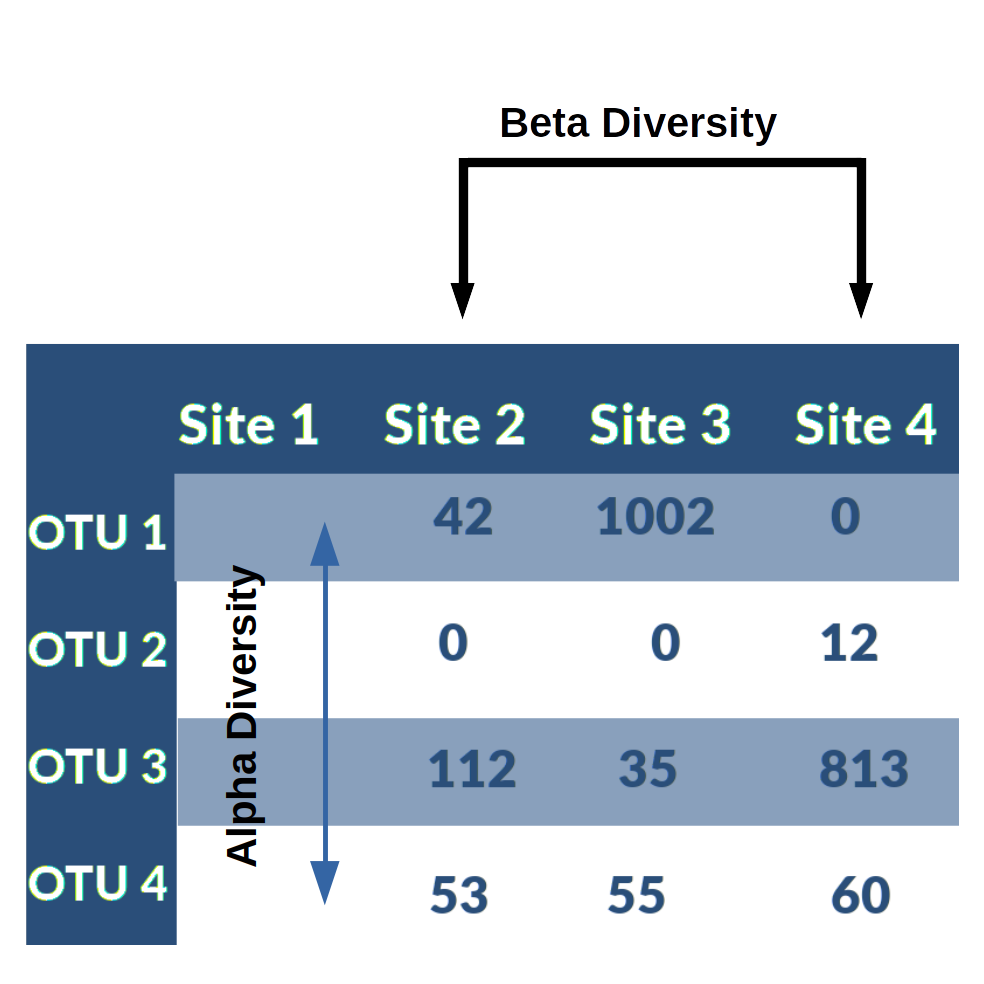
\includegraphics[width=0.5\textwidth]{otutable}
	\caption{An illustration of Alpha and Beta diversity metrics as calculated from OTU tables}
	\label{fig:otu}
\end{figure}

Alpha diversity metrics are a measure of the diversity a sample displays within itself (with respect to the OTUs' reads). An example can be OTU richness which measures the number of OTUs present in the sample (without taking into account the reads) or Shannon index which converts the reads into probabilities (by dividing them with the sample's total reads) and calculates the sample's entropy. The formula is given by:
$$-\sum_{i=1}^s p_i \ln(p_i),$$
were $s$ are the number of species present in the sample, and $p_i$ is the read count of the $i$th OTU divided by the total read count of all OTUs in the sample. 

Beta diversity measures how different samples are in terms of their species composition. They usually take the form of (dis)similarity measures, and some of the more common ones used are Bray-Curtis, Chao and Jaccard (to be explained later). The output of these measures is a symmetric matrix whose elements quantify how (dis)similar the samples are. Ordination methods can then be applied to this matrix that explore its structure graphically. Environmental variables, like pH, concentrations of minerals, or pollutants, can be fitted on top of these plots and help researchers uncover patterns in OTU composition that explain the variables' variation.

If there is a discernible pattern in the ordination plots of the data that separates them along a gradient or grouping of a variable, then differential  abundance analysis can be used to investigate it further. For example, if samples are separated into two groups that also happen to coincide with a categorical variable of the data, a model can be fit to test which OTUs are differentially abundant across the grouping that causes the separation. Parametric models include Zero-Inflated Gaussian mixture model,   Zero-inflated Log-Normal mixture model \cite{css_diff_abund}, and other generalised linear models (like overdispersed Poisson model) \cite{robinson_edger:_2010}. The choice of distributions to model read counts is highly dependent upon the problem and also very debatable \cite{css_diff_abund,white_statistical_2009,mcmurdie_waste_2014}; if their assumptions about the data are not met they can yield a high level of false negatives/positives. 

Non-parametric tests exist that test if groupings of samples (that divides them into two or more groups) result in populations that have significantly different distributions. Such tests include the Mann-Whitney test and permutational multivariate analysis of variance (PERMANOVA). To use such tools the data have to be transformed in some way first, either using alpha or beta diversity. 
%%\textbf{Alpha and Beta Diversity metrics}
%\url{https://www.drive5.com/usearch/manual/diversity_metrics_recommended.html}
%Alpha diversity is the species diversity in a single ecosystem or sample. The simplest measure is richness, the number of species (or OTUs) observed in the sample. Other metrics consider the abundances (frequencies) of the OTUs, for example to give lower weight to lower-abundance OTUs.  
%Beta Diversity measures the differentiation of species diversity between samples or habitats. 
%
%\textbf{Bray–Curtis dissimilarity statistic}:
%In ecology and biology, the Bray–Curtis dissimilarity, named after J. Roger Bray and John T. Curtis,[1] is a statistic used to quantify the compositional dissimilarity between two different sites, based on counts at each site. \url{https://en.wikipedia.org/wiki/Bray%E2%80%93Curtis_dissimilarity}
%	
%	The \textbf{Shannon index} is an information statistic (alpha diversity) that measures diversity of species in a sample. It assumes that all species are represented in the sample and are also randomly sampled. It's equation is given by
%	$$-\sum_{i=1}^s p_i \ln(p_i),$$
%	where $i$ is the index of one of the $s$ species in the sample, and $p_i$ is given by $\frac{n_i}{N}$ where $n_i$ is the number of individuals $i$ in the sample of $N$ individuals.
%	
%	The \textbf{Simpson Index} is a dominance statistic (alpha diversity) that gives more weight to more common species found in the sample. It can be thought as measuring the `effective' number of species and is given by
%	$$\frac{1}{\sum_{i=1}^s p_i^2}$$the value of $p_i$ is defined in  the same way as in the Shannon index.
%	The  \textbf{Jaccard Index} (beta diversity) measures how similar, in terms of species present, two samples are. It ranges from 0 to 1, with the latter indicating that the two samples share the same species. The index does not take into consideration the abundance of species. It is given by
%	$$\frac{|X \cap Y|}{|X\cup Y|},$$
%	where $X$ and $Y$ are two samples, whose intersection is the number of species shared between them and their union is the the total number of species across them.
% Ecological assessments of such surveys have generally been restricted to measuring taxon relative abundances, analyzing within- and between-sample diversity (α and β diversity, respectively), exploring β-diversity patterns using unsupervised learning techniques such as clustering and principal coordinates analysis (PCoA), and performing classical hypothesis testing. These approaches may be limited in their ability to classify unlabeled data or to extract salient features from highly complex and/or sparse data sets. knights et al 2011

%Talk about alpha beta diverrsity and how ordination is used. Also how different abundance testing is done (FitZig) and cite packages used (vegan metagenomeseq DESkati)
%machine learning to characerise biotic index of rivers

\section{Aim}

The aims of this project are to explore the data set obtained from eDNA metabarcoding of samples collected from Peruvian rivers, and use the OTU table to predict the water colour of samples. Data processing techniques like feature selection through correlation and normalisation of the read-counts will be presented in Chapter \ref{chap:data}. These modifications to the OTU table will be used as new features for the classification of samples. Their spatial distribution along the rivers will be taken into account when designing train-validation-test splits; we designed different conditions under which the models'  weaknesses and strengths could be uncovered. These are outlined and explained in the Chapter.

Ordination methods will be used with a variety of distance measures to identify patterns in the data. These methods can also be used for dimensionality reduction, and thus more features will be created for classification. An introduction to the most popular ordination methods will be presented in Section \ref{sec:ordination}. Also, it will be proven that Principal coordinate analysis is a general case of Principal components analysis.

 Permutation Analysis of variance  will be presented in section \ref{sec:permanova}. This classical ecological test hypothesis method  will be used to evaluate if the grouping by water colour divides the samples into populations with significantly different distributions. 

Supervised machine learning models will be trained to predict water colour of samples using a variety of features derived from OTUs. An outline of Bayesian and maximum likelihood logistic regression, as well as of Random forests will be presented in section \ref{sec:classification}. 

These models will then be tested in the ways explained previously, and their performance compared for all the features created. Furthermore, the taxonomic Orders with the most explanatory power will be identified.



%Add packages to all sections like ordination and machne learning
%remove Logistic regression from machine learnig. Start that section with Bayesian framework and then say how logistic regression uses loss functions instead of priors etc.. maybe use AIC as well